
% \begin{savequote}[75mm] 
% Nulla facilisi. In vel sem. Morbi id urna in diam dignissim feugiat. Proin molestie tortor eu velit. Aliquam erat volutpat. Nullam ultrices, diam tempus vulputate egestas, eros pede varius leo.
% \qauthor{Quoteauthor Lastname} 
% \end{savequote}

% \chapter{Consectetuer adipiscing elit}

% \newthought{Lorem ipsum dolor sit amet}, consectetuer adipiscing elit. Morbi commodo, ipsum sed pharetra gravida, orci magna rhoncus neque, id pulvinar odio lorem non turpis. Nullam sit amet enim. Suspendisse id velit vitae ligula volutpat condimentum. Aliquam erat volutpat. Sed quis velit. Nulla facilisi. Nulla libero. Vivamus pharetra posuere sapien. Nam consectetuer. Sed aliquam, nunc eget euismod ullamcorper, lectus nunc ullamcorper orci, fermentum bibendum enim nibh eget ipsum. Donec porttitor ligula eu dolor. Maecenas vitae nulla consequat libero cursus venenatis. Nam magna enim, accumsan eu, blandit sed, blandit a, eros.

% \blindtext

% \section{This is section one}
% \blindtext
% \blindmathpaper

% \section{This is section two}
% \blindtext
% \blindmathpaper
\chapter{Kiến thức nền tảng}
\section{Mạng nơ-ron hồi quy}
\subsection{Dữ liệu tuần tự}
Dữ liệu tuần tự (Sequence data) là loại dữ liệu trong đó thứ tự của các điểm dữ liệu đóng vai trò quan trọng trong việc phân tích và dự đoán. Thông tin tại một thời điểm nhất định không tồn tại độc lập mà có sự phụ thuộc lẫn nhau giữa các thời điểm, thường là thông tin từ quá khứ ảnh hưởng đến tương lai. Dữ liệu tuần tự có thể gặp ở nhiều dạng bài toán khác nhau, từ chuỗi thời gian (time series), văn bản, chuỗi sự kiện, cho đến tín hiệu sinh học. Trong bài toán dự báo giá Bitcoin, dữ liệu tuần tự là dữ liệu giá của Bitcoin theo thời gian, nơi mà giá hiện tại có thể bị ảnh hưởng bởi các giá trước đó. Để xây dựng một mô hình dự báo chính xác, cần có khả năng học được mối quan hệ giữa các giá trong quá khứ và giá hiện tại. Đây là lý do tại sao Recurrent Neural Networks (RNN) trở nên phù hợp để xử lý bài toán này, vì RNN có khả năng ghi nhớ và học từ các dữ liệu tuần tự.
\subsection{Khái niệm}
Mạng nơ-ron hồi quy (Recurrent Neural Networks - RNN) là một loại mạng nơ-ron nhân tạo được thiết kế đặc biệt để xử lý dữ liệu tuần tự, như chuỗi thời gian, văn bản, hoặc tín hiệu âm thanh. Điểm đặc biệt của RNN là khả năng ghi nhớ thông tin từ quá khứ thông qua trạng thái ẩn (hidden state), điều này cho phép mô hình học các phụ thuộc dài hạn trong dữ liệu tuần tự. Tưởng tượng khi ta đang đọc một câu, mỗi từ ta đọc đều có mối liên hệ với các từ trước đó. RNN có khả năng duy trì thông tin này thông qua các bước thời gian, giúp nó trở nên hữu ích cho những bài toán liên quan đến dữ liệu tuần tự.
\subsection{Kiến trúc mạng nơ-ron hồi quy}
Mạng nơ-ron hồi quy (còn được gọi là RNN) là một lớp mạng neural đặc biệt, cho phép sử dụng đầu ra của một bước làm đầu vào cho bước tiếp theo, cùng với việc duy trì trạng thái ẩn qua các thời điểm. Điều này giúp RNN trở nên mạnh mẽ trong việc xử lý các dữ liệu tuần tự và có phụ thuộc lẫn nhau, như chuỗi thời gian hoặc văn bản.

\begin{figure}[h]
    \centering
    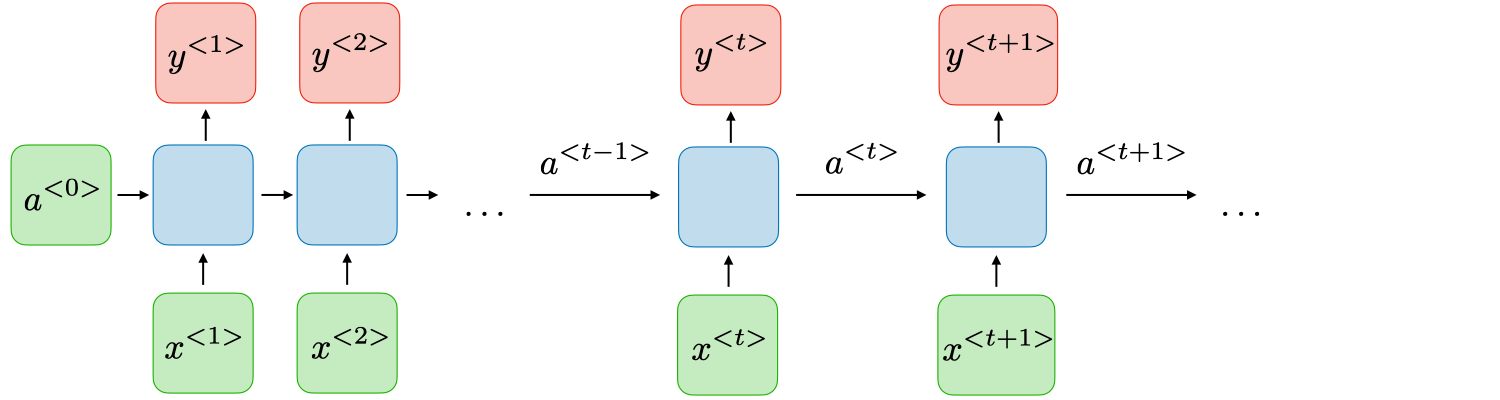
\includegraphics[width=1\textwidth]{images/LSTM/architecture-rnn-ltr.png}
    \caption{Cấu trúc của mạng RNN}
    \label{fig:rnn_architecture}
\end{figure}

Tại mỗi bước $t$, giá trị kích hoạt $a^{\langle t \rangle}$ và đầu ra $y^{\langle t \rangle}$ được biểu diễn như sau:

\begin{equation}
    a^{\langle t \rangle} = g_1 \Big( W_{aa} a^{\langle t-1 \rangle} + W_{ax} x^{\langle t \rangle} + b_a \Big)
\end{equation}

\begin{equation}
    y^{\langle t \rangle} = g_2 \Big( W_{ya} a^{\langle t \rangle} + b_y \Big)
\end{equation}

với $W_{ax}, W_{aa}, W_{ya}, b_a, b_y$ là các hệ số được chia sẻ tạm thời và $g_1, g_2$ là các hàm kích hoạt.

Giải nghĩa các biến
\begin{itemize}
    \item $x^{\langle t \rangle}$: Đầu vào tại thời điểm $t$, ví dụ như một phần của chuỗi dữ liệu.
    \item $a^{\langle t \rangle}$: Trạng thái ẩn tại thời điểm $t$, được tính dựa trên đầu vào hiện tại và trạng thái ẩn trước đó.
    \item $y^{\langle t \rangle}$: Đầu ra tại thời điểm $t$, có thể là giá trị dự đoán của mô hình.
    \item $W_{aa}$: Ma trận trọng số áp dụng cho trạng thái ẩn trước đó.
    \item $W_{ax}$: Ma trận trọng số áp dụng cho đầu vào tại thời điểm hiện tại.
    \item $W_{ya}$: Ma trận trọng số áp dụng cho trạng thái ẩn để tính đầu ra.
    \item $b_{a}$: Bias cho trạng thái ẩn.
    \item $b_{y}$: Bias cho đầu ra.
    \item $g_1, g_2$: Các hàm kích hoạt, ví dụ như hàm sigmoid, tanh hoặc ReLU, được sử dụng để tính toán các giá trị trạng thái ẩn và đầu ra.
\end{itemize}

\begin{figure}[h]
    \centering
    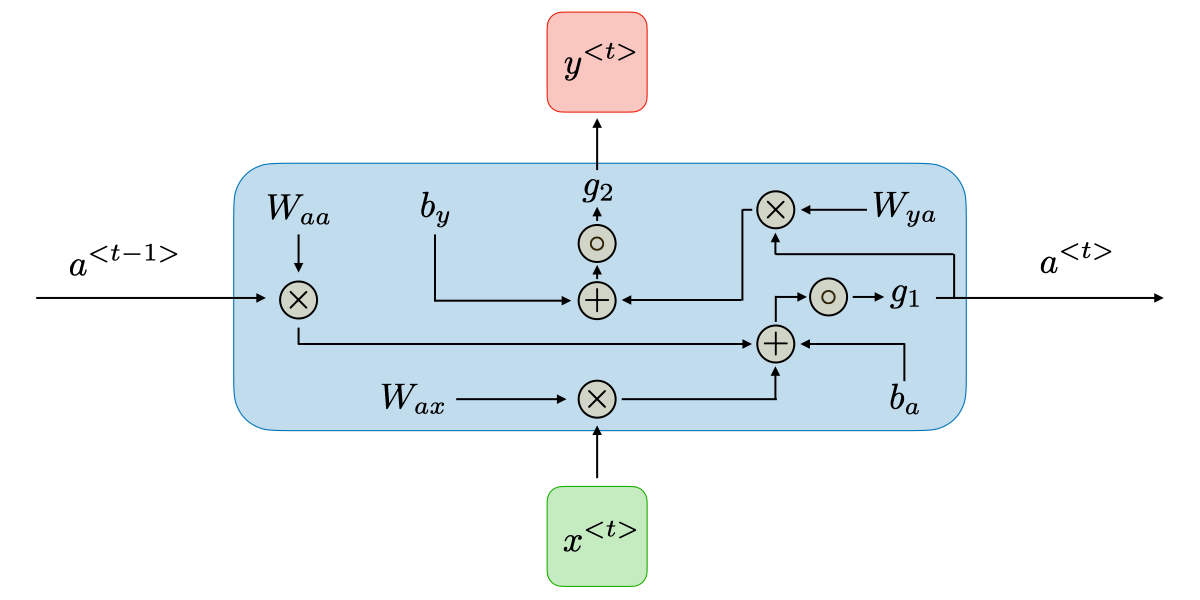
\includegraphics[width=1\textwidth]{images/LSTM/description-block-rnn-ltr.png}
    \caption{Chi tiết cấu trúc của RNN}
    \label{fig:rnn_hidden}
\end{figure}

Các hàm kích hoạt thường dùng trong các modules RNN được miêu tả như sau:

\begin{figure}[h!]
    \centering
    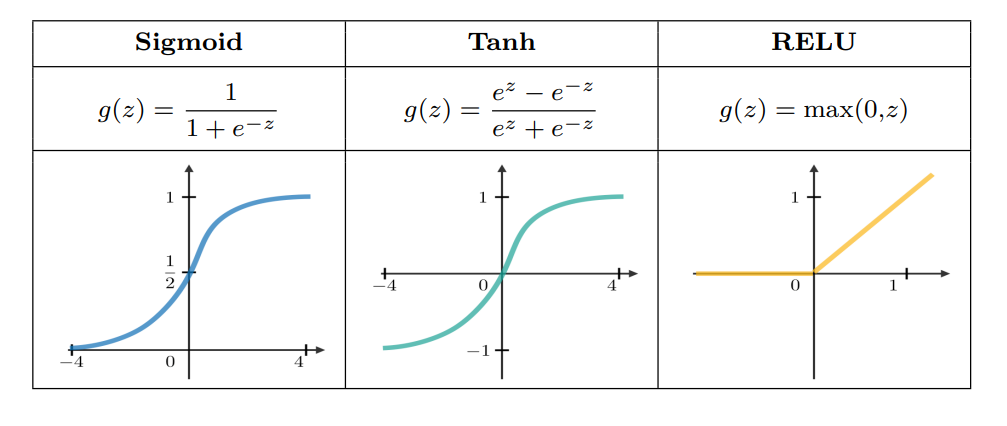
\includegraphics[width=\textwidth]{images/activation.png}
    \caption{Các hàm kích hoạt mà RNN hay sử dụng}
    \label{fig:activation_functions}
\end{figure}

\subsection{Ưu và nhược điểm của RNN}

\begin{table}[h]
    \centering
    \renewcommand{\arraystretch}{1} % tăng khoảng cách giữa các dòng
    \begin{tabular}{|p{7.5cm}|p{7.5cm}|}
        \hline
        \textbf{Ưu điểm} & \textbf{Hạn chế} \\ \hline
        \begin{itemize}
            \item Khả năng xử lí đầu vào với bất kì độ dài nào
            \item Kích cỡ mô hình không tăng theo kích cỡ đầu vào
            \item Quá trình tính toán sử dụng các thông tin cũ
            \item Trọng số được chia sẻ trong suốt thời gian
        \end{itemize} 
        & 
        \begin{itemize}
            \item Tính toán chậm
            \item Khó để truy cập các thông tin từ một khoảng thời gian dài trước đây
            \item Không thể xem xét bất kỳ đầu vào nào trong tương lai cho trạng thái hiện tại
        \end{itemize} \\ \hline
    \end{tabular}
    \caption{Ưu điểm và hạn chế của RNN}
    \label{tab:uudiem_hanche}
\end{table}

\subsection{Hàm mất mát}

Loss Function của RNN bằng tổng các Loss tại các Time-Step:
\begin{equation*}
    \mathcal{L}(\hat{y}, y) = \sum_{t=1}^{T_y} \mathcal{L}(\hat{y}^{\langle t \rangle}, y^{\langle t \rangle})
\end{equation*}

\subsection{Lan truyền ngược theo thời gian}

Lan truyền ngược theo thời gian (Backpropagation) được thực hiện tại mỗi Time-Step. Tại Time-Step $T$, đạo hàm của Loss Function $\mathcal{L}$ đối với ma trận trọng số $W$ được cho bởi công thức:
\begin{equation*}
    \frac{\partial \mathcal{L}^{(T)}}{\partial W} = \sum_{t=1}^{T} \frac{\partial \mathcal{L}^{(T)}}{\partial W}\Big|_{(t)}
\end{equation*}

\subsection{Xử lí phụ thuộc dài hạn}
Vanishing Gradient: Vanishing Gradient xảy ra khi giá trị của gradient trở nên cực kỳ nhỏ trong quá trình lan truyền ngược qua các lớp của mạng neural sâu. Khi gradient trở nên rất nhỏ, các trọng số của mạng không thể cập nhật hiệu quả, điều này khiến cho mạng không học được hoặc học rất chậm. Hiện tượng này đặc biệt phổ biến trong các mạng neural có nhiều lớp hoặc trong các mạng hồi quy (RNN) với chuỗi thời gian dài. Nguyên nhân chính của hiện tượng này là do các gradient bị nhân nhiều lần với các giá trị nhỏ hơn 1, dẫn đến giá trị gần bằng 0 khi chúng lan truyền ngược qua nhiều lớp.

Exploding Gradient: Exploding Gradient xảy ra khi giá trị của gradient trở nên quá lớn trong quá trình lan truyền ngược, dẫn đến sự cập nhật trọng số không ổn định hoặc thậm chí gây tràn số (overflow). Điều này làm cho mạng trở nên không ổn định và không thể hội tụ, thường xảy ra khi các gradient được nhân nhiều lần với các giá trị lớn hơn 1 qua nhiều lớp. Để khắc phục vấn đề này, một kỹ thuật thường được sử dụng là Gradient Clipping, nhằm giới hạn giá trị của gradient trong một phạm vi nhất định, giúp đảm bảo quá trình học của mạng được ổn định hơn.

Giống như nhiều mô hình học sâu khác, hiện tượng Vanishing và Exploding Gradient cũng xuất hiện trong RNN, gây khó khăn cho việc ghi nhớ các trạng thái từ những bước thời gian xa. Nguyên nhân chính của vấn đề này là do việc nhân gradient theo hàm mũ, dẫn đến sự tăng hoặc giảm đột ngột khi số lượng lớp mạng tăng lên, khiến quá trình học trở nên không ổn định.

Sử dụng ReLU chúng ta đã giải quyết được khá tốt vấn đề Vanishing Gradient. Còn đối với Exploring Gradient, chúng ta có thể sử dụng Gradient Clipping.

\begin{figure}[h!]
    \centering
    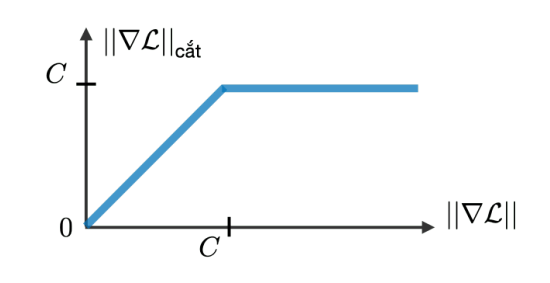
\includegraphics[width=0.8\textwidth]{images/gradient.png}
    \caption{Gradient Clipping để giới hạn Gradient}
    \label{fig:gradient_clipping}
\end{figure}

Gradient clipping là một kĩ thuật được sử dụng để giải quyết vấn đề exploding gradient xảy ra khi thực hiện lan truyền ngược. Bằng việc giới hạn giá trị lớn nhất cho gradient, hiện tượng này sẽ được kiểm soát trong thực tế.

\section{Bộ nhớ dài-ngắn hạn (LSTM)}
Bộ nhớ dài-ngắn hạn (Long Short Term Memory) là một phiên bản cải tiến của RNN, giúp mô hình dễ dàng ghi nhớ dữ liệu quá khứ hiệu quả hơn. Với LSTM, vấn đề Vanishing Gradient trong RNN được giải quyết tốt hơn, nhờ đó mô hình có khả năng lưu giữ và học từ thông tin ở các bước thời gian xa. LSTM đặc biệt phù hợp cho các bài toán phân loại, xử lý, và dự đoán chuỗi thời gian có độ dài không cố định. Mô hình này cũng được huấn luyện thông qua quá trình Backpropagation.

Kiến trúc của mạng LSTM bao gồm nhiều lớp (Layers), mỗi lớp được cấu thành từ các đơn vị nhỏ gọi là Cell. Mỗi Cell được mô tả bởi hai bộ nhớ quan trọng: Cell State (\(C\)) và Hidden State (\(h\)).

- \textbf{Hidden State - h,H}: Bộ nhớ ngắn hạn (\textit{working memory}), lưu giữ thông tin từ Cell ngay trước Cell hiện tại. Hidden State tồn tại trong cả RNN và LSTM, và cũng chính là Output của mỗi Cell trong RNN/LSTM.

- \textbf{Cell State - C}: Bộ nhớ dài hạn (\textit{long-term memory, memory cell}), có nhiệm vụ lưu trữ thông tin từ nhiều Cells trong quá khứ. Bộ nhớ này chỉ tồn tại trong LSTM, giúp mạng duy trì thông tin cần thiết qua các bước thời gian.

Xét một Cell tại thời điểm hiện tại (\(C_t, h_t\)) trong LSTM, luồng dữ liệu đi qua Cell này sẽ lần lượt trải qua ba cổng chính như sau:

- \textbf{Forget gate}: Cổng này quyết định thông tin nào từ Cell trước đó (\(C_{t-1}\)) cần được giữ lại hay loại bỏ. Thông tin từ Hidden State trước (\(h_{t-1}\)) và từ Input hiện tại (\(x_t\)) được đưa qua hàm Sigmoid, tạo ra một giá trị từ 0 đến 1. Giá trị càng gần 0 cho thấy thông tin ít quan trọng và có thể bỏ qua, trong khi giá trị càng gần 1 cho thấy thông tin quan trọng cần được giữ lại.

\begin{figure}[h!]
    \centering
    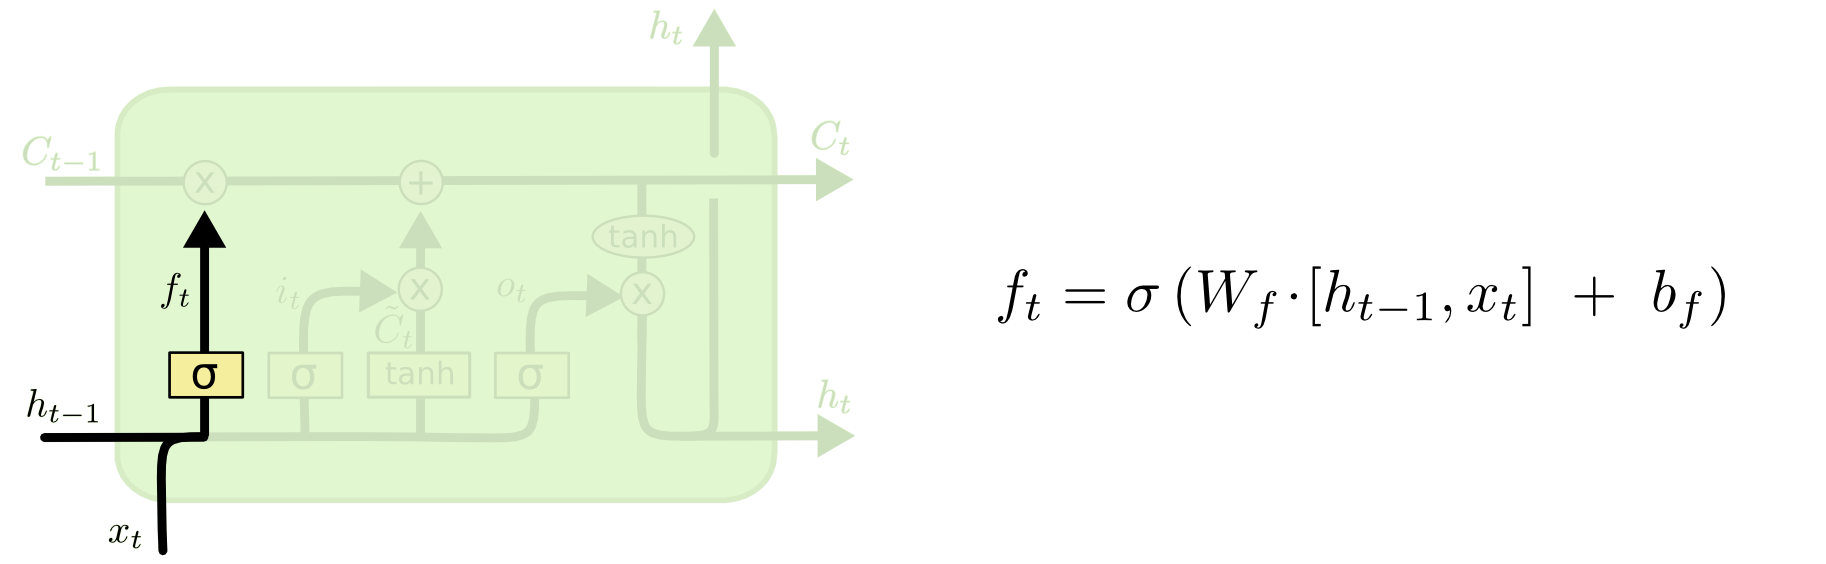
\includegraphics[width=\textwidth]{images/LSTM/lstm-forget-f.png}
    \caption{Minh họa Forget Gate trong LSTM}
    \label{fig:lstm_cell}
\end{figure}

\begin{equation*}
    f_t = \sigma \left( W_f \cdot [h_{t-1}, x_t] + b_f \right) = \sigma (W_{xf} X_t + W_h h_{t-1} + b_f)
\end{equation*}

- \textbf{Input gate}: Cổng này quyết định giá trị nào từ Hidden State trước (\(h_{t-1}\)) và thông tin từ Input hiện tại (\(x_t\)) sẽ được đưa vào Cell hiện tại. Để thực hiện điều này, cổng sử dụng kết hợp hai hàm Sigmoid và Tanh. Tương tự như Forget Gate, thông tin từ Hidden State trước (\(h_{t-1}\)) và từ Input hiện tại (\(x_t\)) được đưa qua hàm Sigmoid, tạo ra một giá trị từ 0 đến 1, phản ánh mức độ quan trọng của thông tin—càng gần 0 thì thông tin càng ít quan trọng, càng gần 1 thì thông tin càng quan trọng. Tiếp theo, hàm Tanh tạo ra một vector ứng cử cho Cell State hiện tại (\(\tilde{C_t}\)). Output từ hai hàm này được nhân với nhau để tính toán Cell State của thời điểm hiện tại.


\begin{figure}[h!]
    \centering
    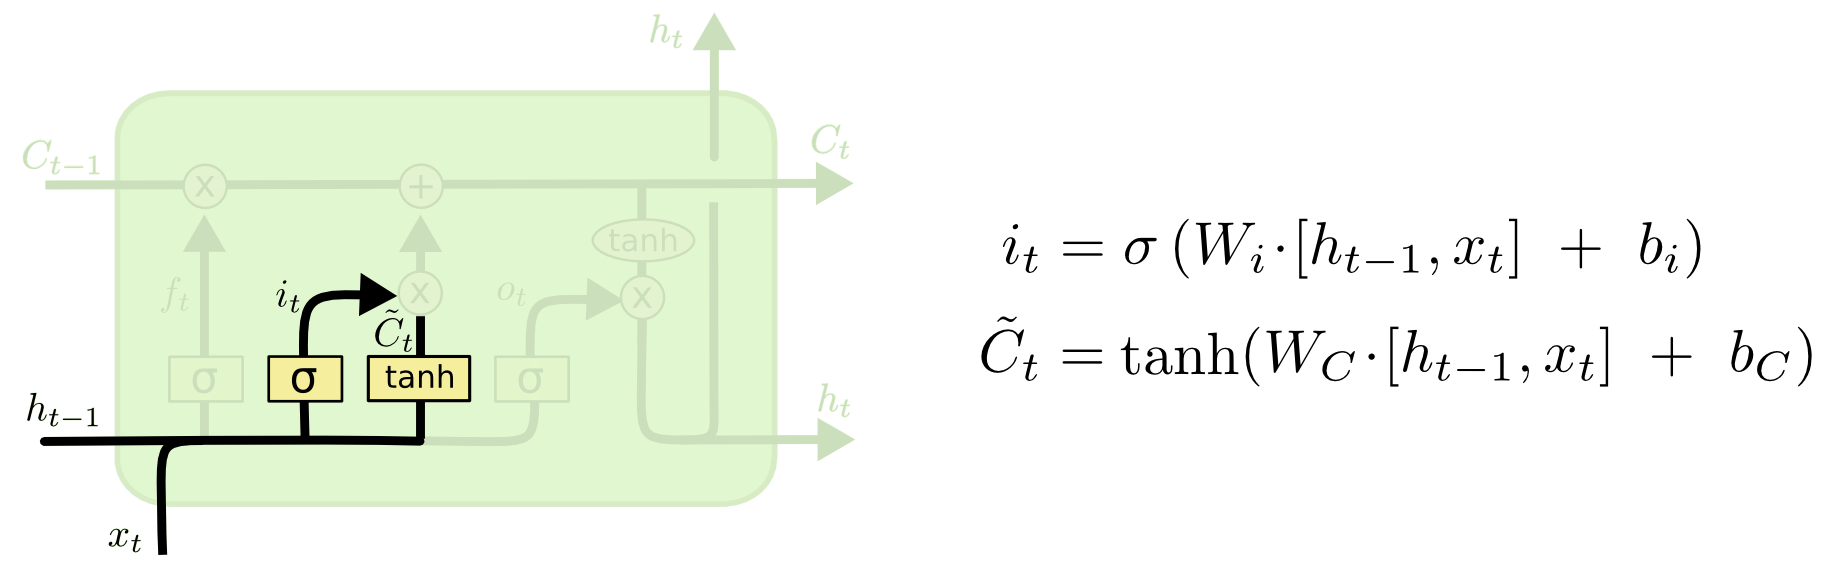
\includegraphics[width=\textwidth]{images/LSTM/lstm-input-i.png}
    \caption{Minh họa Input Gate trong LSTM}
    \label{fig:lstm_input_gate}
\end{figure}

\begin{equation*}
    i_t = \sigma \left( W_i \cdot [h_{t-1}, x_t] + b_i \right) = \sigma (W_{xi} X_t + W_h h_{t-1} + b_i)
\end{equation*}

\begin{equation*}
    \tilde{C_t} = \tanh \left( W_c \cdot [h_{t-1}, x_t] + b_c \right) = \tanh (X_t W_{xc} + h_{t-1} W_{hc} + b_c)
\end{equation*}

Đến đây, ta đã có thể tính được Cell State hiện tại:

\begin{figure}[h!]
    \centering
    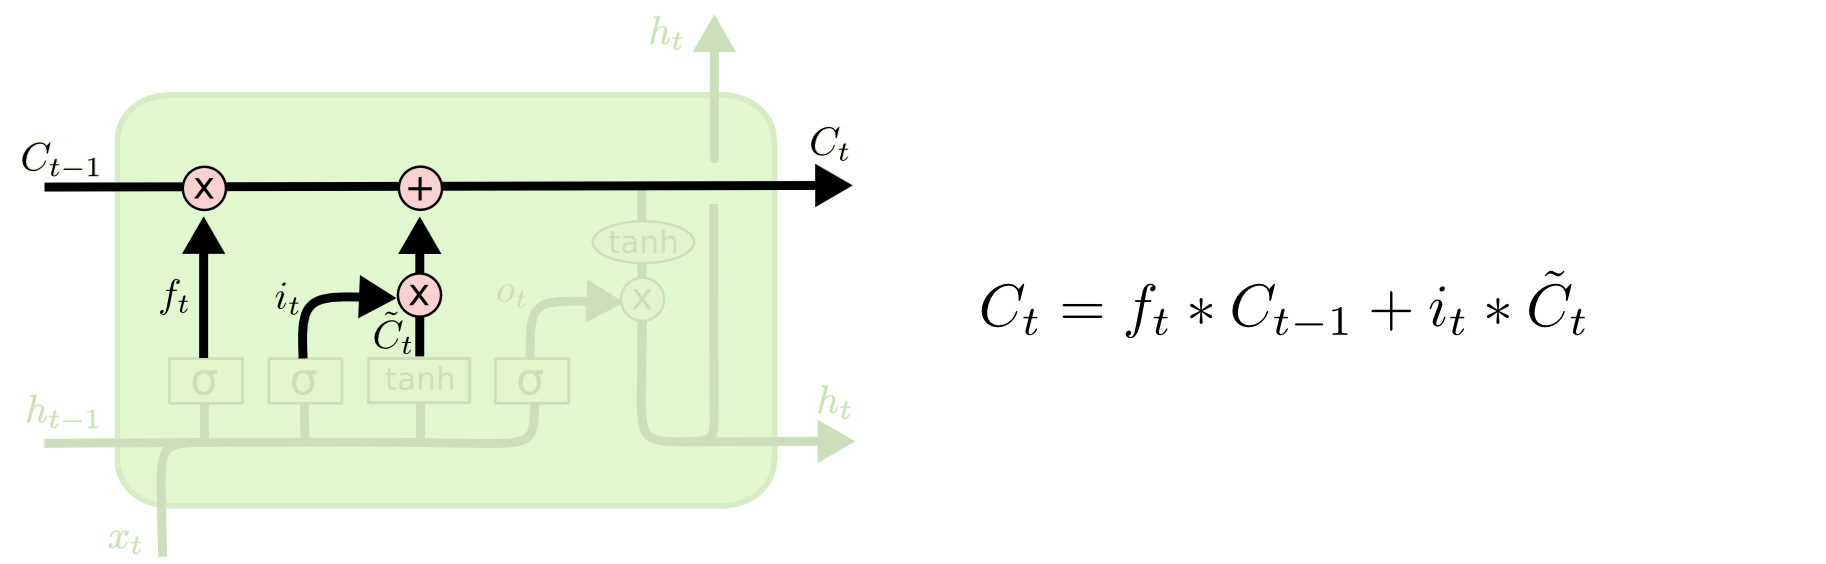
\includegraphics[width=\textwidth]{images/LSTM/lstm-cellstate-c.png}
    \caption{Minh họa tính toán Cell State hiện tại}
    \label{fig:lstm_cell_state}
\end{figure}

\begin{equation*}
    C_t = f_t * C_{t-1} + i_t * \tilde{C_t}
\end{equation*}

Chú giải về các phép toán:

\begin{itemize}
    \item \(\otimes\): Element-wise multiplication
    \item \(\oplus\): Element-wise addition
\end{itemize}

Chúng ta nhân trạng thái của Cell trước đó với \(f_t\) rồi cộng với \(i_t * \tilde{C_t}\):

\begin{equation*}
    C_t = f_t * C_{t-1} + i_t * \tilde{C_t}
\end{equation*}

- \textbf{Output gate}: Cổng này xác định thông tin nào sẽ được truyền ra làm đầu ra (\(h_t\)). Tương tự như hai cổng trước đó, thông tin từ Hidden State trước (\(h_{t-1}\)) và từ Input hiện tại (\(x_t\)) được đi qua hàm Sigmoid, tạo ra một giá trị từ 0 đến 1. Giá trị này càng gần 0 thì thông tin càng kém quan trọng, ngược lại, giá trị càng gần 1 cho thấy thông tin càng quan trọng. Sau đó, Cell State được chuyển qua hàm Tanh để đưa giá trị về khoảng \([-1, 1]\).

\begin{figure}[h!]
    \centering
    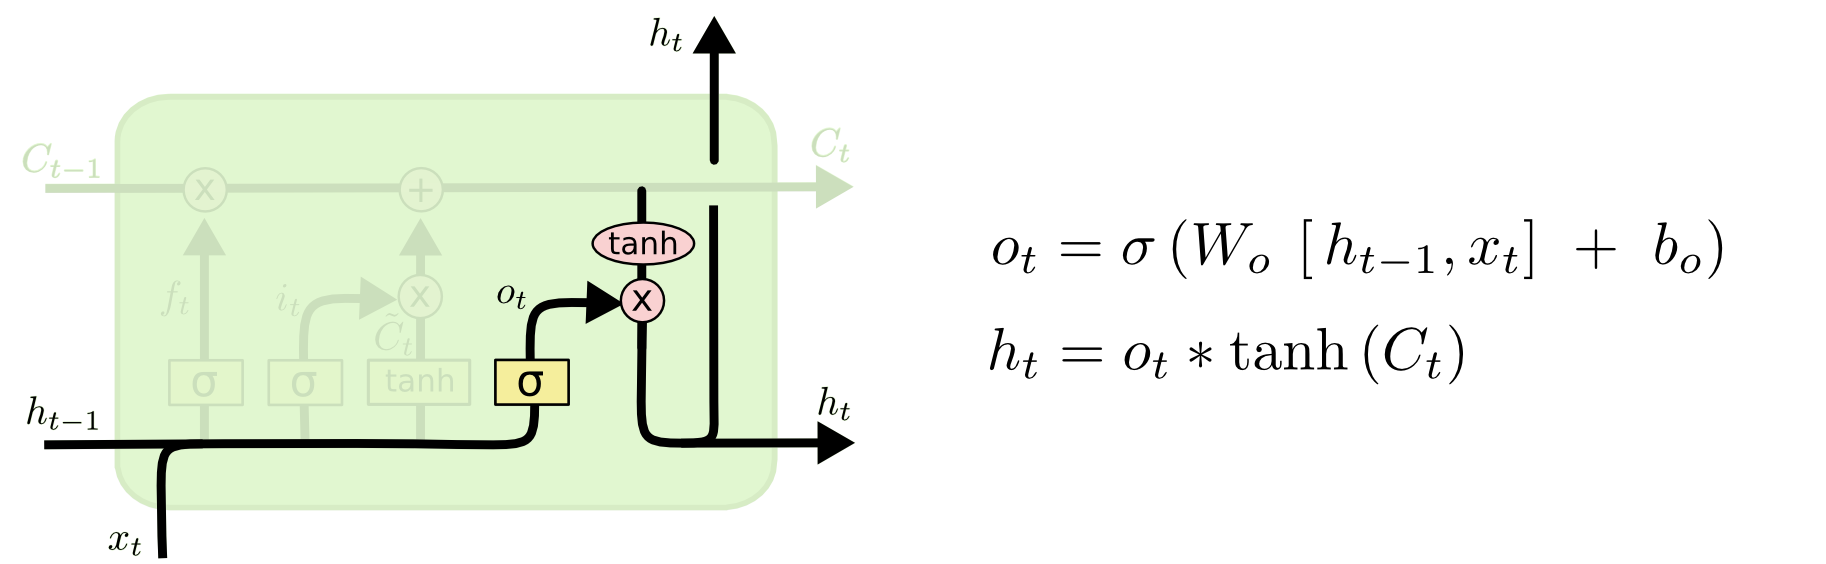
\includegraphics[width=\textwidth]{images/LSTM/lstm-output-o.png}
    \caption{Minh họa Output Gate trong LSTM}
    \label{fig:lstm_output_gate}
\end{figure}

Output của Cell được tính như sau:

\begin{equation*}
    o_t = \sigma \left( W_o \cdot [h_{t-1}, x_t] + b_o \right) = \sigma (W_{xo} X_t + W_h h_{t-1} + b_o)
\end{equation*}

\begin{equation*}
    h_t = o_t * \tanh (C_t)
\end{equation*}

\section{Gated Recurrent Unit (GRU)}
Gated Recurrent Unit (GRU) là một phiên bản cải tiến khác của RNN, được phát triển nhằm giải quyết vấn đề Vanishing Gradient và tăng hiệu suất học của mạng. GRU có cấu trúc đơn giản hơn LSTM khi chỉ sử dụng hai cổng: Reset Gate và Update Gate. Nhờ thiết kế tinh gọn này, GRU thường yêu cầu ít tài nguyên tính toán hơn nhưng vẫn đạt được hiệu quả tương đương với LSTM trong nhiều trường hợp. Điều này giúp GRU trở thành lựa chọn phù hợp cho các bài toán yêu cầu khả năng xử lý nhanh hoặc trên các thiết bị có hạn chế về tài nguyên.

\begin{figure}[h!]
    \centering
    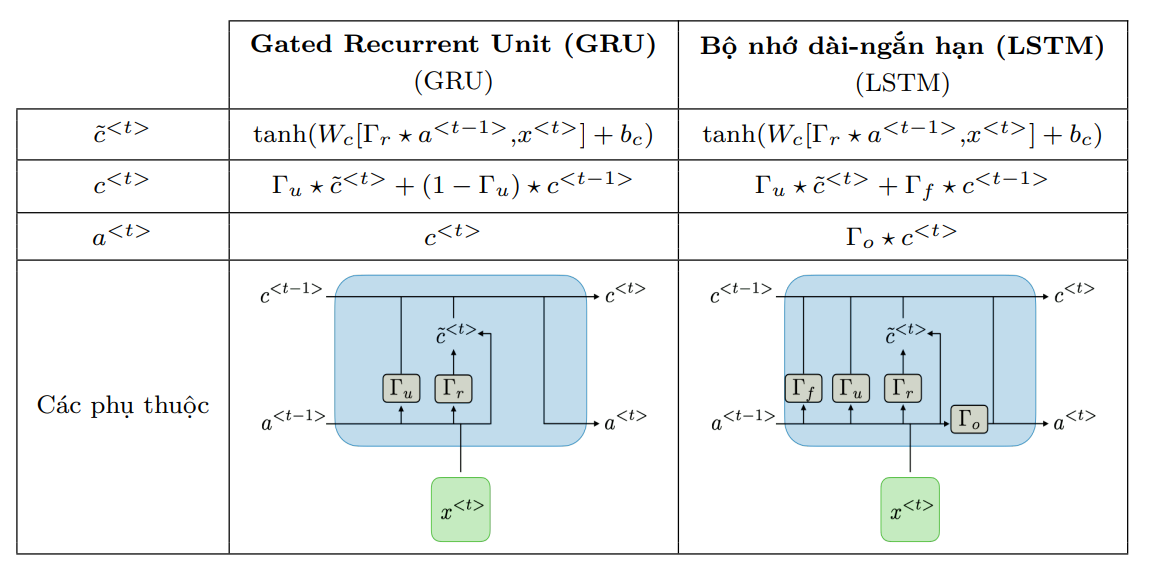
\includegraphics[width=0.7\textwidth]{images/LSTM/lstm_summary.png}
    \caption{Tổng kết các phương trình đặc trưng của LSTM và GRU}
    \label{fig:lstm_summary}
\end{figure}







% Phần cây quyết định và rừng ngẫu nhiên (chưa thêm ảnh và chưa link phương trình, chưa có reference)
\section{Cây quyết định}

\subsection{Giới thiệu}
Cây quyết định là một mô hình có cấp bậc (hierarchichal) có giám sát (supervised), trong đó những vùng cục bộ được xác định bằng việc chia ra một cách hồi quy.
Cây quyết định gồm có 2 thành phần chính: nút quyết định (decision nodes) và các lá kết thúc (terminal leaves).
Mỗi nút quyết định $m$ chứa một hàm thử $f_m(\mathbf{x})$ với kết quả rời rạc được đánh nhãn cho các nhánh.
\begin{figure}[hbpt]
    \centering
    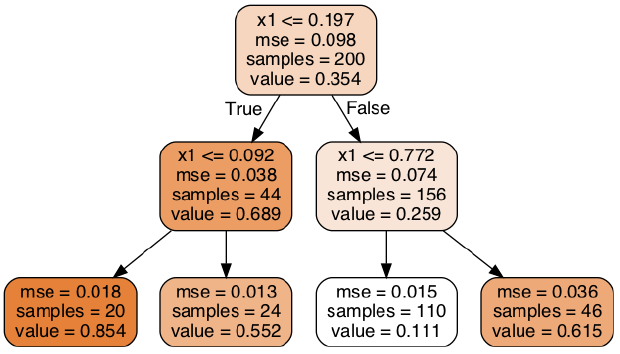
\includegraphics[width=\linewidth]{figures/decision_tree.png}
    \caption{Ví dụ về một cây quyết định}
    \label{fig:decision_tree_example}
\end{figure}

\subsection{Cây đơn biến}
Mỗi nút trong cây đơn biến \textbf{chỉ sử dụng một biến (feature / attribute) trong chiều dữ liệu đầu vào.} Đây cũng là cài đặt mặc định của \textit{scikit-learn} \cite{aurelien2019handsonml}.
\begin{itemize}
    \item Nếu biến được sử dụng, ký hiệu $x_j$ là rời rạc thì nút sẽ sử dụng một trong số $n$ giá trị rời rạc đó và nhánh đó sẽ có khả năng được chia ra thành $n$ nhánh con (gọi là $n$-way split).
    \item Nếu biến được sử dụng là biến số thì nó nên được rời rạc hóa, nhưng nếu là số có thứ tự (liên tục) thì phép thử được sử dụng sẽ là phép so sánh, và vì vậy nó là 2-way split.
\end{itemize}

\begin{equation} f_m(\mathbf{x}): x_j - w_{m0} > 0 \end{equation}

\subsection{Cây phân loại}
Với cây phân loại thì chất lượng của mỗi lần chia nhánh sẽ được đo bằng \textit{độ hỗn loạn}. Độ hỗn loạn càng thấp thì tức là lần chia nhánh càng tốt.
Trong một nút $m$, ta ký hiệu $N_m$ là số lượng phần tử trong tập huấn luyện đã cập đến nút $m$ (Với nút gốc thì $N_{root} = N$), $N^i_m$ trong số $N_m$ thuộc về lớp $C_i$. Một phần tử trong tập huấn luyện cập đến nút $m$ thì xác suất để nó thuộc lớp $C_i$ là

\begin{equation} \hat{P}(C_i|\mathbf{x}, m) \equiv p^i_m = \frac{N^i_m}{N_m} \end{equation}

Nút $m$ thuần khi $p^i_m$ với tất cả mọi $i$ là 0 hoặc 1 (tức là xác suất để vào các lớp là 0 hoặc 1). 0 khi không có phần tử thuộc lớp $C_i$ nào cập đến nút $m$, và 1 khi tất cả đều cập đến nút $C_i$. Nếu nút ổn định thì ta không cần chia thêm nút con (nhánh con) cho nó nữa. Một cách để đo độ hỗn loạn là \textit{entropy} - được tính theo công thức sau:

\begin{equation} I_m = -\sum_{i = 1}^{K} {p^i_m \log_2(p^i_m)} \end{equation}

\begin{figure}
    \centering
    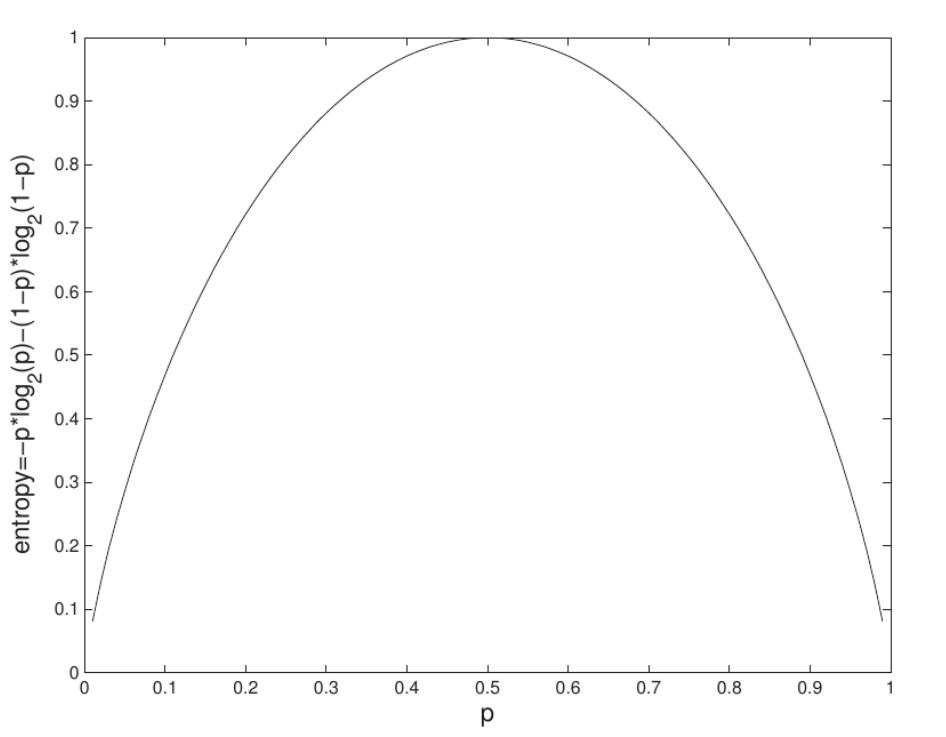
\includegraphics[width=\linewidth]{figures/entropy_graph.png}
    \caption{Đồ thị của hàm entropy}
    \label{fig:entropy_graph}
\end{figure}


Một đô đo sự hỗn loạn khác cũng được sử dụng phổ biến là chỉ số Gini:

\begin{equation} \phi(p, 1 - p) = 2p(1-p) \end{equation}

Nếu nút $m$ không thuần, thì mẫu dữ liệu cần được chia nhỏ để giảm độ hỗn loạn, và ta sẽ có phương án chia tùy thuộc vào dữ liệu. Trong các phương án được xét, ta cần tìm cách để giảm thiểu được độ hỗn loạn, để cho các nhánh sau ta không cần chia thêm nhiều lần nữa. Tất nhiên đây chỉ là \textbf{tối ưu cục bộ}, và ta không thể đảm bảo tìm ra được cây nhỏ nhất.
Ví dụ, ở nút $m$, $N_{mj}$ trong số $N_m$ phần tử theo nhánh $j$, đây là các phần tử $\mathbf{x}^t$ mà kết quả của phép thử $f_m(\mathbf{x}^t)$ trả về kết quả $j$. \textit{Đối với thuộc tính rời rạc với $n$ lớp, ta sẽ có $n$ kết quả; với một thuộc tính số, ta sẽ có 2 kết quả và giả sử có $n$ phần tử thì sẽ có $n - 1$ khe để ta có thể chia chúng thành hai tập}; cả hai trường hợp đều thỏa mãn $\sum_{j=1}^{n} N_{mj} = N_m$. $N^i_{mj}$ trong số $N_{mj}$ phần tử thuộc về lớp $C_i$: $\sum_{i=1}^{K} N^{i}_{mj} = N_{mj}$. Tương tự, $\sum_{j=1}^{n} N^i_{mj} = N^i_m$.

Cho nút $m$, kết quả của phép thử là $j$, vậy xác suất một phần tử được xác định vào lớp $C_i$ là:

\begin{equation} \hat{P}(C_i|\mathbf{x}, m, j) \equiv p^i_{m, j} = \frac{N^i_{m, j}}{N_{m, j}} \end{equation}

và độ hỗn tạp sau khi chia nhánh là:

\begin{equation} I'_m = -\sum^n_{j=1}\frac{N_{mj}}{N_m} \sum_{i = 1}^{K} {p^i_{mj} \log_2(p^i_{mj})} \end{equation}

Dưới đây là mã giả dạng Python để ta có thể hình dung ra được cách xây dựng một cây quyết định từ tập đầu vào \cite{alpaydin2010introml}:

\begin{algorithm}[H]
    \caption{Decision Tree Generation}
    \SetKwFunction{GenerateTree}{GenerateTree}
    \SetKwFunction{SplitAttribute}{SplitAttribute}
    \SetKwFunction{SplitEntropy}{SplitEntropy}
    \SetKwFunction{NodeEntropy}{NodeEntropy}
    \SetKwProg{Fn}{Function}{:}{}
    
    \Fn{\GenerateTree{$X$}}{
        \eIf{\NodeEntropy{X} $< \theta_i$}{
            Create leaf labeled by majority class in $X$\;
            \Return\;
        }{
            $i \gets$ \SplitAttribute{$X$}\;
            \For{each branch of $x_i$}{
                Find $X_i$ falling in branch\;
                \GenerateTree{$X_i$}\;
            }
        }
    }
    
    \Fn{\SplitAttribute{$X$}}{
        $minEntropy \gets \infty$\;
        \For{all attributes $i = 1$ to $d$}{
            \If{$x_i$ is discrete with $n$ values}{
                Split $X$ into $X_1, \ldots, X_n$ by $x_i$\;
                $e \gets$ \SplitEntropy{$X_1, \ldots, X_n$}\;
                \If{$e < minEntropy$}{
                    $minEntropy \gets e$\;
                    $bestF \gets i$\;
                }
            }
            \If{$x_i$ is numeric}{
                \For{all possible splits}{
                    Split $X$ into $X_1, X_2$ on $x_i$\;
                    $e \gets$ \SplitEntropy{$X_1, X_2$}\;
                    \If{$e < minEntropy$}{
                        $minEntropy \gets e$\;
                        $bestF \gets i$\;
                    }
                }
            }
        }
        \Return $bestF$\;
    }
\end{algorithm}

Vậy là với mỗi thuộc tính, rời rạc hay liên tục, phân mục hay số, thì ta sẽ tìm ra cách phân chia làm cho entropy trở nên nhỏ nhất. Đây là cơ sở của thuật toán cây phân loại và hồi quy (Classification And Regression Tree - CART).

\subsection{Cây hồi quy}
Cây hồi quy được xây dựng tương tự như cây phân loại, thay vì sử dụng độ hỗn loạn thì ta sẽ sử dụng một độ đo khác làm thang đo cho việc phân nhánh.
Giả sử trong nút $m$, $X_m$ là tập con của $X$ cập đến nút $m$ (tức là các phần tử được phân vào nút $m$ khi duyệt qua cây).

\begin{equation} b_m(x) = \begin{cases} 1 & \text{if } x \in X_m: \, x \text{ cập đến nút  } m\\ 0 & \text{ngược lại} \end{cases} \end{equation}

Trong cây hồi quy, chất lượng của một lần chia nhánh sẽ được đo bằng trung bình sai số bình phương (Mean Squared Error). Nếu ta ký hiệu $g_m$ là giá trị được ước lượng cho nút m thì

\begin{equation} E_m = \frac{1}{N_m} \sum_t{(r^t - g_m)^2 \cdot b_m(\mathbf{x}^t)} \end{equation}

Với $N_m = |{X_m}| = \sum_t{b_m(\mathbf{x}^t)}$.
Phương trình (6) sẽ thể hiện phương sai của kết quả thực với đầu ra trong nút $m$.
Trong một nút, ta dùng trung bình của các kết quả đầu ra (trung vị nếu có quá nhiều nhiễu)

\begin{equation} g_m = \frac{\sum_t {b_m (x_t)r^t}}{\sum_t {b_m (x_t)}} \end{equation}

Nếu tại một nút, sai số là chấp nhận được (tức là $E_m < \theta_r$ nào đó) thì một nút lá sẽ được tạo ra và lưu $g_m$ lại nút lá đó.
Nếu sai số không đạt yêu cầu, thì dữ liệu cập đến nút m sẽ tiếp tục được phân chia sao cho tổng sai số cho từng nhánh là thấp nhất. Giống với cây phân loại, ta sẽ đi tìm cách chia một thuộc tính nào đó sao cho sai số trung bình là nhỏ nhất, và tiếp tục công việc đó với các nhánh con.
Giả sử $X_{mj}$ là tập con của $X_m$ theo nhánh $j$. $\bigcup_{j=1}^{n} X_{mj} = X_{m}$ (tức là hội của phần tử theo mỗi nhánh $j$ từ $1$ đến $n$ sẽ là tập hợp các phần tử (tập mẹ) đạt đến nhánh $m$).
Ta định nghĩa

\begin{equation} b_{mj}(x) = \begin{cases} 1 & \text{if } x \in X_{mj}: \, x \text{ cập đến nút  } m \text {  và theo nhánh j}\\ 0  & \text{ngược lại} \end{cases} \end{equation}

$g_{mj}$ là giá trị được ước lượng cho nhánh $j$ của nút $m$.

\begin{equation} g_{mj} = \frac{\sum_t {b_{mj} (x_t)r^t}}{\sum_t {b_{mj} (x_t)}} \end{equation}

Và sai số sau khi chia nhánh là

\begin{equation} E'_m = \frac{1}{N_m}\sum_j \sum_t{(r^t - g_{mj})^2 \cdot b_{mj}(\mathbf{x}^t)} \end{equation}

Độ suy giảm sai số của một nhánh được chỉ ra ở phương trình (6) và (10). Ta sẽ đi tìm cách phân nhánh nào mà sai số ở phương trình (10) là nhỏ nhất. Trong đoạn mã giả mô phỏng, \texttt{node\_entropy(X)} và \texttt{split\_entropy([X])} sẽ được thay bằng việc tính toán sai số bình phương trung bình.

Vấn đề khi đặt ra ngưỡng sai số hoặc ngưỡng ổn định của dữ liệu $\theta_i$, ta phải chọn một mức phù hợp vì khi $\theta_i$ nhỏ thì sai số sẽ phải nhỏ và mô hình sẽ xảy ra tình trạng quá khớp (overfitting) và nếu đặt ở ngưỡng quá cao thì mô hình sẽ trở nên không hiệu quả (underfitting).

Một cách để giải quyết vấn đề là ta cắt tỉa các nút (tức là hủy phân nhánh nữa) - được đề cập ở phần tiếp theo.
\begin{figure}
    \centering
    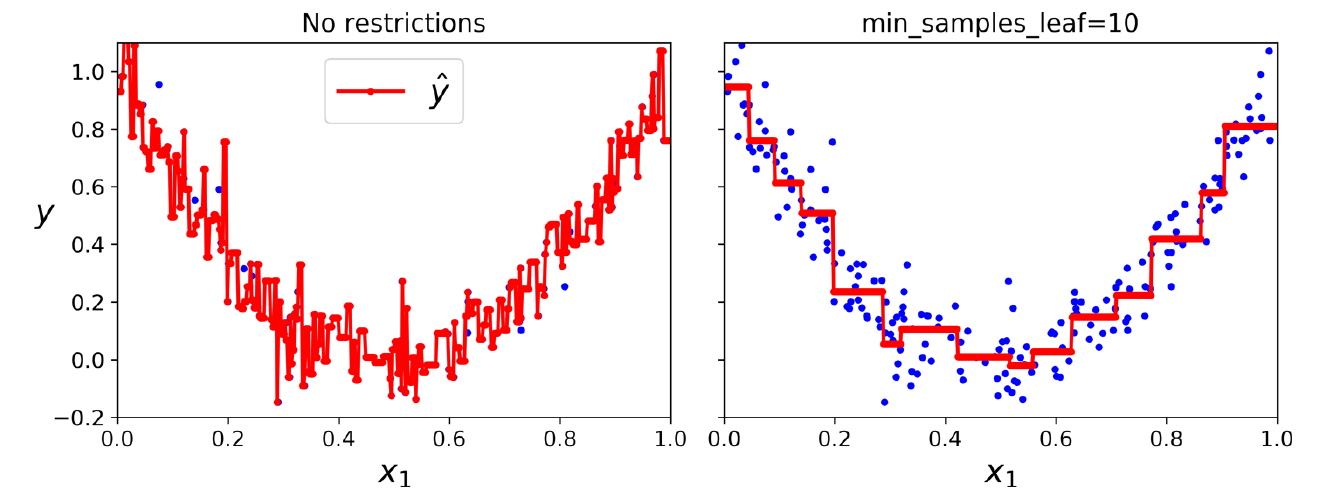
\includegraphics[width=\linewidth]{figures/dt_overfit1.png}
    \caption{Hình minh họa về việc overfitting ở cây quyết định khi độ sâu không bị giới hạn}
    \label{fig:dt_overfit1}
\end{figure}
\begin{figure}
    \centering
    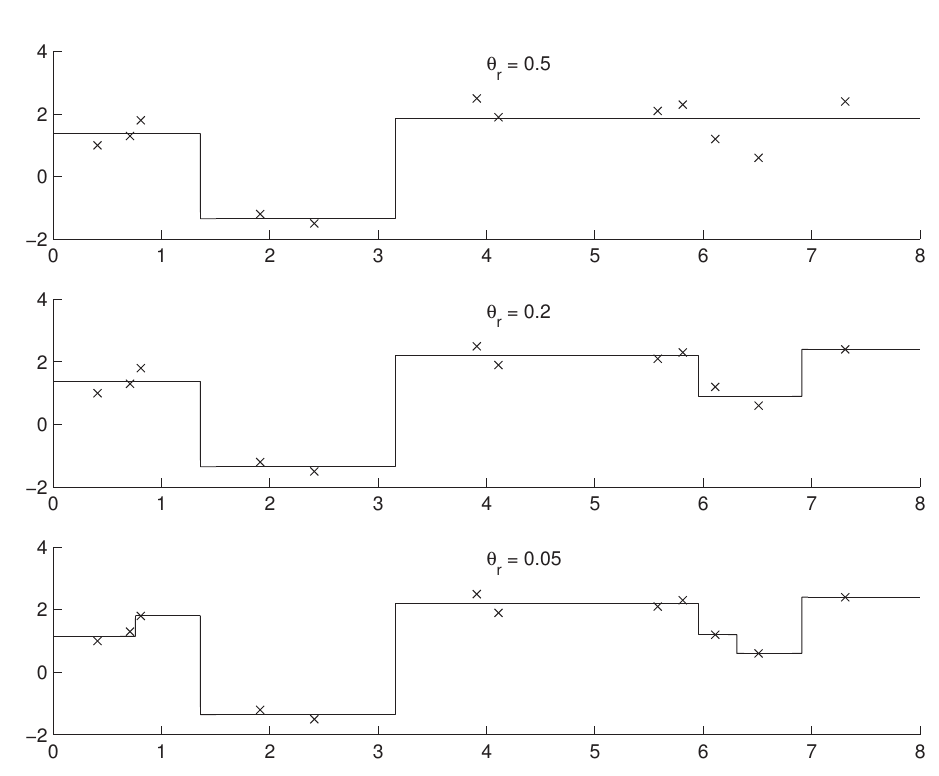
\includegraphics[width=0.7\linewidth]{figures/dt_overfit2.png}
    \caption{Hình minh họa fitting ở cây quyết định khi $\theta$ được đặt với nhiều giá trị khác nhau}
    \label{fig:dt_overfit2}
\end{figure}
\subsection{Cắt tỉa - Pruning}
Thường thì một nút sẽ không được chia nhỏ thêm nếu số lượng mẫu huấn luyện đến nút đó nhỏ hơn một tỷ lệ nhất định của tập huấn luyện - ví dụ, 5 phần trăm - bất kể độ không thuần hay sai số. Ý tưởng ở đây là bất kỳ quyết định nào dựa trên quá ít mẫu sẽ gây ra sự biến động và do đó làm tăng lỗi tổng quát hóa. Việc dừng quá trình xây dựng cây sớm trước khi cây được hoàn thiện được gọi là \textbf{cắt tỉa sớm (prepruning)}.
Một phương pháp để có được cây đơn giản hơn là \textbf{cắt tỉa sau (postpruning)}, điều này trên thực tế \textit{hoạt động hiệu quả hơn} so với cắt tỉa sớm (prepruning). Chúng ta đã thấy trước đó rằng quá trình xây dựng cây là tham lam, và ở mỗi bước, chúng ta đưa ra một quyết định, cụ thể là tạo ra một nút quyết định và tiếp tục mà không quay lại để thử các lựa chọn thay thế. Ngoại lệ duy nhất là \textbf{cắt tỉa sau (postpruning)}, trong đó chúng ta cố gắng tìm và cắt tỉa những nhánh con không cần thiết.

Với cắt tỉa sau, ta sẽ cho phép cây phát triển đầy đủ, đến khi tất cả các lá kết thúc đều thuần và không xuất hiện lỗi huấn luyện. Sau đó, ta sẽ tìm các cây con gây ra hiện tượng quá khớp và cắt tỉa chúng. Từ tập huấn luyện ban đầu, ta sẽ tạo thêm một \textbf{tập cắt tỉa} (pruning set) không dùng cho huấn luyện. Với mỗi cây con (nút con bên trong cây quyết định), thay thế nó bằng một lá nhãn. \textit{Lá này được gắn nhãn với lớp phổ biến nhất (trung bình với bài toán hồi quy) của các mẫu dữ liệu được phân loại vào cây con đó}. Nếu lá nhãn không hoạt động kém hơn cây con trên tập cắt tỉa, chúng ta cắt tỉa cây con và giữ lá nhãn; nếu không, chúng ta giữ cây con.

\subsection{Cây đa biến}
\textbf{Cây quyết định đơn biến} chỉ sử dụng một chiều đầu vào tại mỗi điểm phân chia. Trong \textbf{cây quyết định đa biến}, tại một nút quyết định, tất cả các chiều đầu vào có thể được sử dụng, do đó nó tổng quát hơn. Khi tất cả các đầu vào đều ở dưới dạng số, một \textbf{nút đa biến tuyến tính nhị phân} được định nghĩa là

\begin{equation} f_m(\mathbf{x}): \mathbf{w}_m^t\mathbf{x} + w_{m0} > 0 \end{equation}

Vì nút đa biến tuyến tính lấy tổng trọng số nên các thuộc tính rời rạc nên được mã hóa thành 0/1.
Tuy nhiên, một khó khăn mà ta gặp phải nữa, đó là ở một nút quyết định thì ta sẽ có rất nhiều cách chọn thuộc tính và giá trị thuộc tính để có thể chia nhánh. Ví dụ nếu tập dữ liệu có $d$ thuộc tính, và ta có $N_m$ phần tử cập đến nút m, thì khi quyết định chia ta sẽ có $2^d$ cách chọn thuộc tính, và với mỗi cách chọn thuộc tính ta lại có $\binom{N_m}{d}$ cách chia tập dữ liệu thành các khoảng. Vì vậy tìm kiếm thủ công là không khả thi. Một trong các giải pháp đã được đề cập là thuật toán OC1 \cite{Murthy1993oc1}.

\section{Rừng ngẫu nhiên - Random Forest}
Đây là một phương pháp học kết hợp các cây quyết định, và hầu hết được huấn luyện theo phương pháp tổng hợp khởi động có lặp (bootstrap aggregating - bagging) hoặc tổng hợp không thay thế (pasting). Vậy bagging và pasting có nghĩa là gì?
Trong \textbf{Bagging}, các tập dữ liệu con được chọn ngẫu nhiên từ tập dữ liệu gốc \textbf{có phép thay thế} (tức là một mẫu có thể xuất hiện nhiều lần trong các tập con). Sau đó, một mô hình riêng biệt được huấn luyện trên từng tập dữ liệu con, và kết quả cuối cùng được tổng hợp lại (\textit{trung bình đối với các bài toán hồi quy hoặc bỏ phiếu đa số đối với các bài toán phân loại}).
Lợi ích của Bagging là giảm phương sai của mô hình và cải thiện độ chính xác bằng cách tận dụng nhiều mô hình độc lập. Với Bagging, thống kê chỉ ra rằng, vì có những phần tử dữ liệu được chọn lại nên sẽ có lên đến 37\% dữ liệu chưa bao giờ được đưa vào huấn luyện\cite{aurelien2019handsonml}, và vì thế ta có thể đánh giá độ chính xác của mô hình này trên tập dữ liệu này 
\textbf{Pasting} cũng tương tự như \textbf{Bagging}, nhưng khác biệt quan trọng là các tập dữ liệu con được chọn \textbf{không có phép thay thế} (tức là một mẫu không thể xuất hiện nhiều lần trong các tập con). Quá trình huấn luyện và tổng hợp kết quả cũng giống Bagging, nhưng do không có phép thay thế, các tập con sẽ có xu hướng khác nhau hoàn toàn.
Pasting hữu ích khi muốn mỗi mẫu dữ liệu chỉ xuất hiện một lần trong một tập con, để đảm bảo đa dạng hơn cho các mô hình con.
Cài đặt mặc định của scikit-learn cho rừng ngẫu nhiên hồi quy sẽ là bagging\cite{aurelien2019handsonml}.

Ngoài ra, với các cây trong rừng ngẫu nhiên, thay vì tìm kiếm vị trí và thuộc tính tốt nhất trong tập tất cả thuộc tính để chia nhánh, \textit{chúng vẫn tìm kiếm vị trí và thuộc tính tốt nhất nhưng mà là trong một tập hợp con ngẫu nhiên của các thuộc tính}. Điều này tạo ra sự đa dạng của các cây, đánh đổi độ lệc lấy phương sai. Nhìn chung, đây là một đánh đổi có lợi, giúp tạo ra một mô hình tổng thể tốt hơn.

\section{Thuật toán tăng cường độ dốc cực đại (XGBoost)}

\section{Stacking}